\documentclass{article}
\usepackage[utf8]{inputenc}

\title{Final Report for Cooking Project}
\author{sep team }
\date{August 2020}

\usepackage{natbib}
\usepackage{graphicx}

\begin{document}

\maketitle

\section{Introduction}
About 10 years ago, recipes could be found in magazines, or on television shows.
Then we jot them down by copying them, making general notes, or buying books about recipes at the bookstore.\\
With the growth of the internet recently, we can easily search for recipes that are shared online, or cooking communities willing to share them online.\\
However, with the development of mobile technology, the need to manage separate recipes anytime, anywhere with personal phones, even without the network, has increased, users always want to store recipes. and can be found easily.\\
Or you can store the recipe photos, then write down the steps to create a recipe for yourself right on your phone instead of having to write them down in notes like before.
When you love the recipes, users need to be able to search the recipes online, and then import them to their phone to easily store them. \\
That's why the team decided to create an application to manage these recipes, which would be a store for every recipe or the word "Master-Chief" or "Jan-Can-Cook" just with a small phone.

Team  
* Tran Huy Phuc
* Nguyen Chi Cong 
* Phan Hoang Huy

\begin{figure}[h!]
\centering
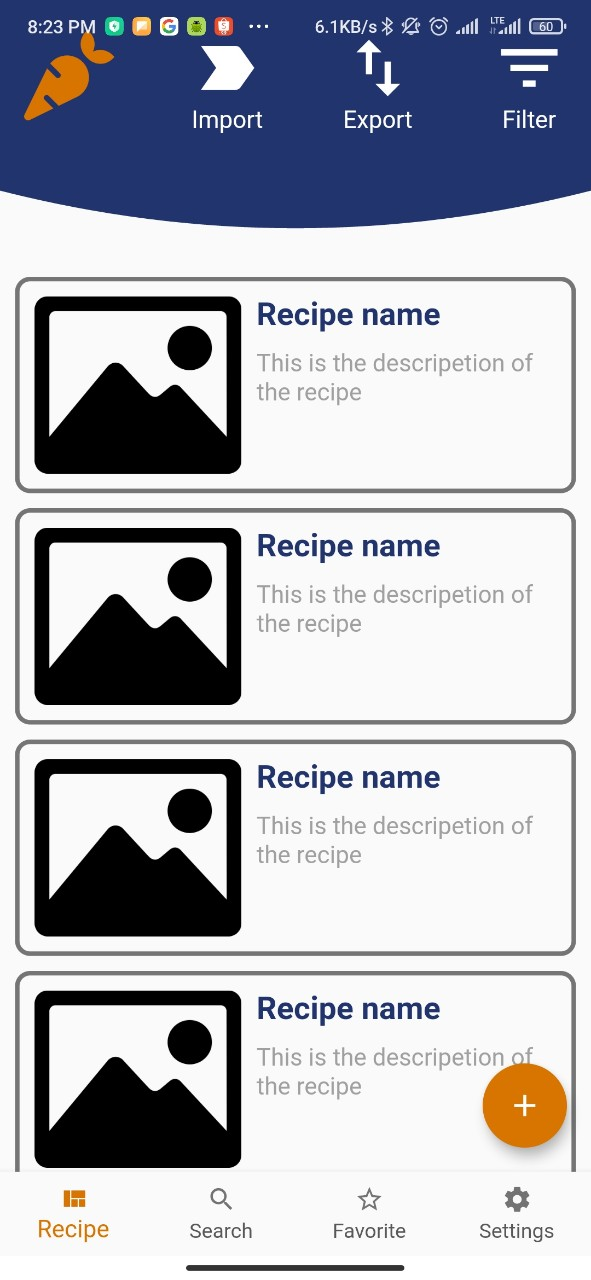
\includegraphics[scale=0.1]{CookingBook.jpg}
\caption{Cooking Book}
\label{fig:cookingbook}
\end{figure}

\section{Project Details }

\subsection{Software Engineering introduction}


\subsubsection{Software qualities}


\subsubsection{ Architecture and tests}
\subsubsection {Frontend (Mobile app) }
\\
a. Framework: \\
We only consider cross-platform frameworks: React Native (https://reactnative.dev) or Flutter (https://flutter.dev). The reasons behind this decision are: \\
o Afteranalizingtherequirements(bothnon-functionalandfunctional requirements), we concluded that the application does not require any specific native function that cross-platform framework can not do.\\
o Wedon’thaveenoughtimeandresourcestobuildandmantain2separate code bases (one for Android and one for iOS).\\
After we finished our reasearch (visit their official website and documentation, read many articles (listed in references 4a. at the end of this document)), we ended up to choose Flutter for this project, because:\\
o Flutterhasbetterperformance(evenbetternativeinafewcases).\\
o Flutterhasbetterdocumentation. \\
o FlutterisbeingdevelopedandmantainedbyGoogleofficially,whileReact native is not supported officially by Facebook anymore. \\
o FlutterwillsupportwebandPC(andprobablyotherplatformsinthefuture). \\
o Programming language: We chose Flutter, so Dart is the programming language we will use. \\

\subsubsection{Backend}
As user wants to import a list of Recipe or search a Recipe in the internet, we have: 2.1. A Backend API for search recipe (provided by team, and host it In cloud) ( Code by .net core 2.0, and host it in AWS EC2, and it contains 1 SECRET KEY selected by team). All recipe needs to manual insert into database, it can be store by MySQL. 2.2. Use 3rd party API for example: Edamam Nutrition Analysis, or Tasty API.
6
There are 2 main function from each API: List/Search recipe by a criterion Get details of a recipe
All response data need to be json format but have different fields (depended by API provider). And front-end code needs to convert this format into standard structure data.
A Recipe json result example as below :
\begin{lstlisting}[language=Python, caption=Python example]
import numpy as np
{
"title": "Fresh Ham Roasted With Rye Bread and Dried Fruit Stuffing", "prep": "1. Have your butcher bone and butterfly the ham and score
the fat in a diamond pattern. ...", "yield": "About 15 servings", "ingr": [
"1 fresh ham, about 18 pounds, prepared by your butcher (See Step 1)",
"7 cloves garlic, minced",
"1 tablespoon caraway seeds, crushed",
"4 teaspoons salt",
"Freshly ground pepper to taste",
"1 teaspoon olive oil",
"1 medium onion, peeled and chopped",
"3 cups sourdough rye bread, cut into 1/2-inch cubes",
"1 1/4 cups coarsely chopped pitted prunes",
"1 1/4 cups coarsely chopped dried apricots",
"1 large tart apple, peeled, cored and cut into 1/2-inch cubes", "2 teaspoons chopped fresh rosemary",
"1 egg, lightly beaten",
"1 cup chicken broth, homemade or low-sodium canned"
] 
-}
\end{lstlisting}

\subsubsection{References} 
\textbf{React native vs. Flutter } \\
- https://www.thedroidsonroids.com/blog/flutter-vs-react-native-what-to-choose-in-
2020 \\
- https://nevercode.io/blog/flutter-vs-react-native-a-developers-perspective/ \\
- https://medium.com/@adhithiravi/react-native-vs-flutter-what-are-the-differences-
b6dc892f0d34 \\
- https://medium.com/@moqod_development/flutter-vs-react-native-for-cross- platform-development-821b44138b4a \\
- https://medium.com/swlh/flutter-vs-native-vs-react-native-examining-performance- 31338f081980 \\
\textbf{Flutter documentation: }  \\
https://flutter.dev/docs \\
\subsubsection{Unit test}:
Built-in test package of Flutter (https://flutter.dev/docs/cookbook/testing/unit/introduction)
“Mock”: use mockito (https://flutter.dev/docs/cookbook/testing/unit/mocking)
CI (continuous integration): Github action
When we merge code from any branch to “master” branch, pre-define script on Github action will be triggerred to run all the tests. If the tests are passed, it continues to build .apk file and stores it on Github (we probably send this apk to Slack channel if we need).
State management in Flutter: We use mobX (https://mobx.netlify.com) because of its simplicity.\\
\subsubsection{Acceptance test}:
For project, we design different functions such as: Import, Export, Filter, Recipe, Search, Favorite, and Setting.
-Import function
There is one annoucement for clicking it. 
-Export function
-Filter function
-Recipe function
The user interface will be shown product lists. The user is easy to look and choose all food names on cooking application
-Search function
-Favorite function
-Setting function



\subsubsection{ Bibliography, existing analysis }
\subsubsection{existing analysis}

\begin{itemize}
\item 1. Recipe book
\item 2. Recipe website.
\item 3. Recipe App : My cook book manager
\item 4. Recipe online app. :Tasty
\end{itemize}


\begin{center}
 \begin{tabular}{||c c c c c||} 
 \hline
  & Recipe Book & Recipe Website & Recipe App & Recipe Online App \\ [0.5ex] 
  & (Magnolia Table) & (allrecipes.com) & (My cook book manager) & (Tasty) \\ [0.5ex] 
 \hline\hline
My own recipe & No & No & Yes & Yes \\ 
 \hline
 Search recipe & No & yes & yes & yes \\
 \hline
 easy to use & no & no, need account & yes & yes \\
 \hline
 cost & costly & free & free &  costly\\
 \hline
 internet & No & Require & no & Require \\ [1ex] 
 \hline
  Import, Export & No & no & yes & no \\ [1ex] 
 \hline
\end{tabular}
\caption{Table 1.  Compare kind of existing cook book}
\end{center}

\subsection{scientific approach}

\subsection{ Requirements analysis and objective}
\subsubsection{ Usecase diagram}

\begin{figure}[h!]
\centering
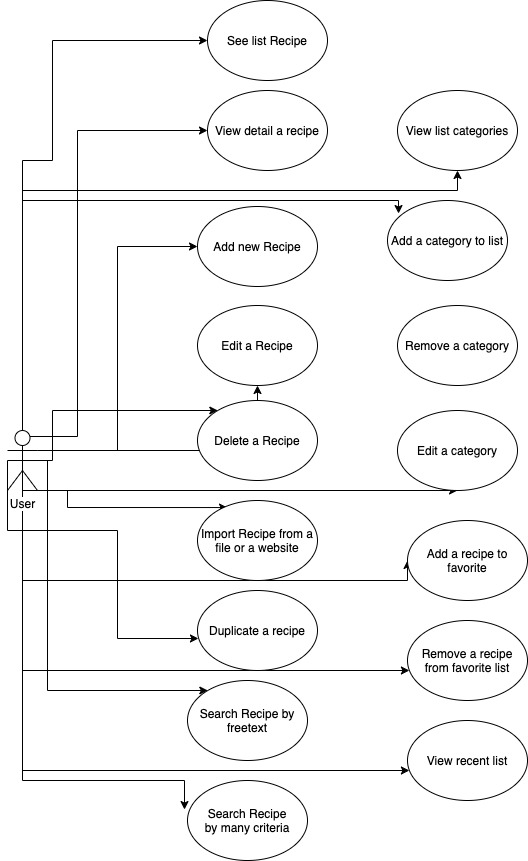
\includegraphics[scale=0.5]{Usecase.jpg}
\caption{Usecase - diagram}
\label{fig:Usecase}
\end{figure}

\subsubsection{ Functional Requirement}
\begin{enumerate}
\item  Recipe list:User can view their recipe list on homepage. Each item on the list shows recipe basic information (name, image, short description). \\
\item Sort recipes: user can sort their recipes in different orders(Ex:name, created date), default order is name. 
\item Create new recipe: user has the ability to create new recipe from the app.
\item View recipe details: user can click on any recipe on the recipe list to view its details.
\item Edit recipe: user is able to edit existing recipe and save updated details to database.
\item Delete recipe: user can delete an existing recipe. A popup dialog should be shown to user to confirm the deletion. After deleted, the recipe will be removed our of local database and disappears on recipe list.
\item  Duplicate recipe: user can use this function to clone an existing recipe to new one quickly.
\item Import recipes: user is able to use the app to import one or more recipes from the file that was exported before. User can import recipes from the internet too.
\item Export recipes: from the app, user can export one or more recipes to a file. This file can be shared to other users or re-imported to the app later.
\item Search recipe(s): user can search recipe(s) from local database or remote database.
\item Category list: user can view list of categories. Click on a category to view all the recipes belong to that category.
\item Create new category: from the app, user can create new category (with name and description).
\item Edit category: user is able to edit the information of category.
\item Delete category: user is able to delete existing categories. A popup dialog should be shown to user to confirm the deletion. After deleted, the deleted category will no longer be shown in category list.
\item Favorite recipes: user can add any recipe to favorite list, so that user can find these recipes faster.
\item Remove recipes out of favorite list: user is able to remove recipes out of the favorite list. A popup dialog should be shown to user to confirm the removal.
\item Push notification: user can receive notifications (if they allow)
\item Resume Application: When they're an action with higher priority ( like phone call ), the application should pause, and resume all progress when the action is finished.

\end{enumerate}



\subsubsection{ Non-Functional Requirement}
\begin{enumerate}
\item \textbf{Performance/Storage} : Storage of application if acceptance ( < 100Mb )
\item \textbf{Performance/Response} : All local response action must < 1s.
\item \textbf{Performance/Memory} : Memory of application if acceptance for an manage application ( < 100Mb Memory when running ).
\item \textbf{Responsiveness}: with any “unexpected event” from user, like a phone call, or user press home button, the application still works fine, and resumes after the event has completed. 
\item \textbf{Portability} : User can export all user information data from a device and move it into another devices or share it to anywhere. With install file ( or download it from store ), user can re-import all export data.
\item \textbf{Fiability} : When there's an error, or wrong action from user, it will display user friendly message ( like images must less than 2Mb ) instead of a system message ( like buffer is overload ).
\item \textbf{Scalibilit} : The app is designed and developed to be able to handle at least thousands of recipes. 
\item \textbf{Usability} : there’re no “hidden function” that very complex to use or complex to find. 
\item \textbf{Accessibility} : All functions need to have less than 5 steps, normal should be 3 steps. 
\item \textbf{Reliability} : All the function need to work probably. If there is any wrong action from user, the app should be inform error to user. For any search recipe outside the internet ( use 3rd party API ), make sure return value must be correct and does not break any function. 
\item \textbf{Screen Adaption}: Support the most popular mobile screen size from 4.0 inch to 7.0 inch. Able to render its layouts on different screen sizes. Along with automatic adjustment of font size and image rendering. 
\item \textbf{Modifiable} : The application can be changed easily when 3rd party API has been stop or update structure. 
\item \textbf{Security}: There’re no user data, or any sensitive data store by application, or publish into internet. 
\item \textbf{Maintainability} : Application written by Flutter (widely supported by community and easy to learn). There’re document and comment code for any function/class. There’re no function/class more than 2000 lines code. 
\item \textbf{Compatibility} : support the most used platforms today on android platform and ios :  Minimum supported Android version: the application is able to run on Android 5.0 and up.  Minimum supported IOS version: the application is able to run on iOS 10 and up. 
\item \textbf{Localized} : The app supports English but also has the ability to support other languages easily. 
\item \textbf{Version control ability} : All code and documents store with control version on GitHub, that we can manage the version of all code/documents 
\end{enumerate}

\subsubsection{ Mock-up}

\begin{figure}[h!]
\centering
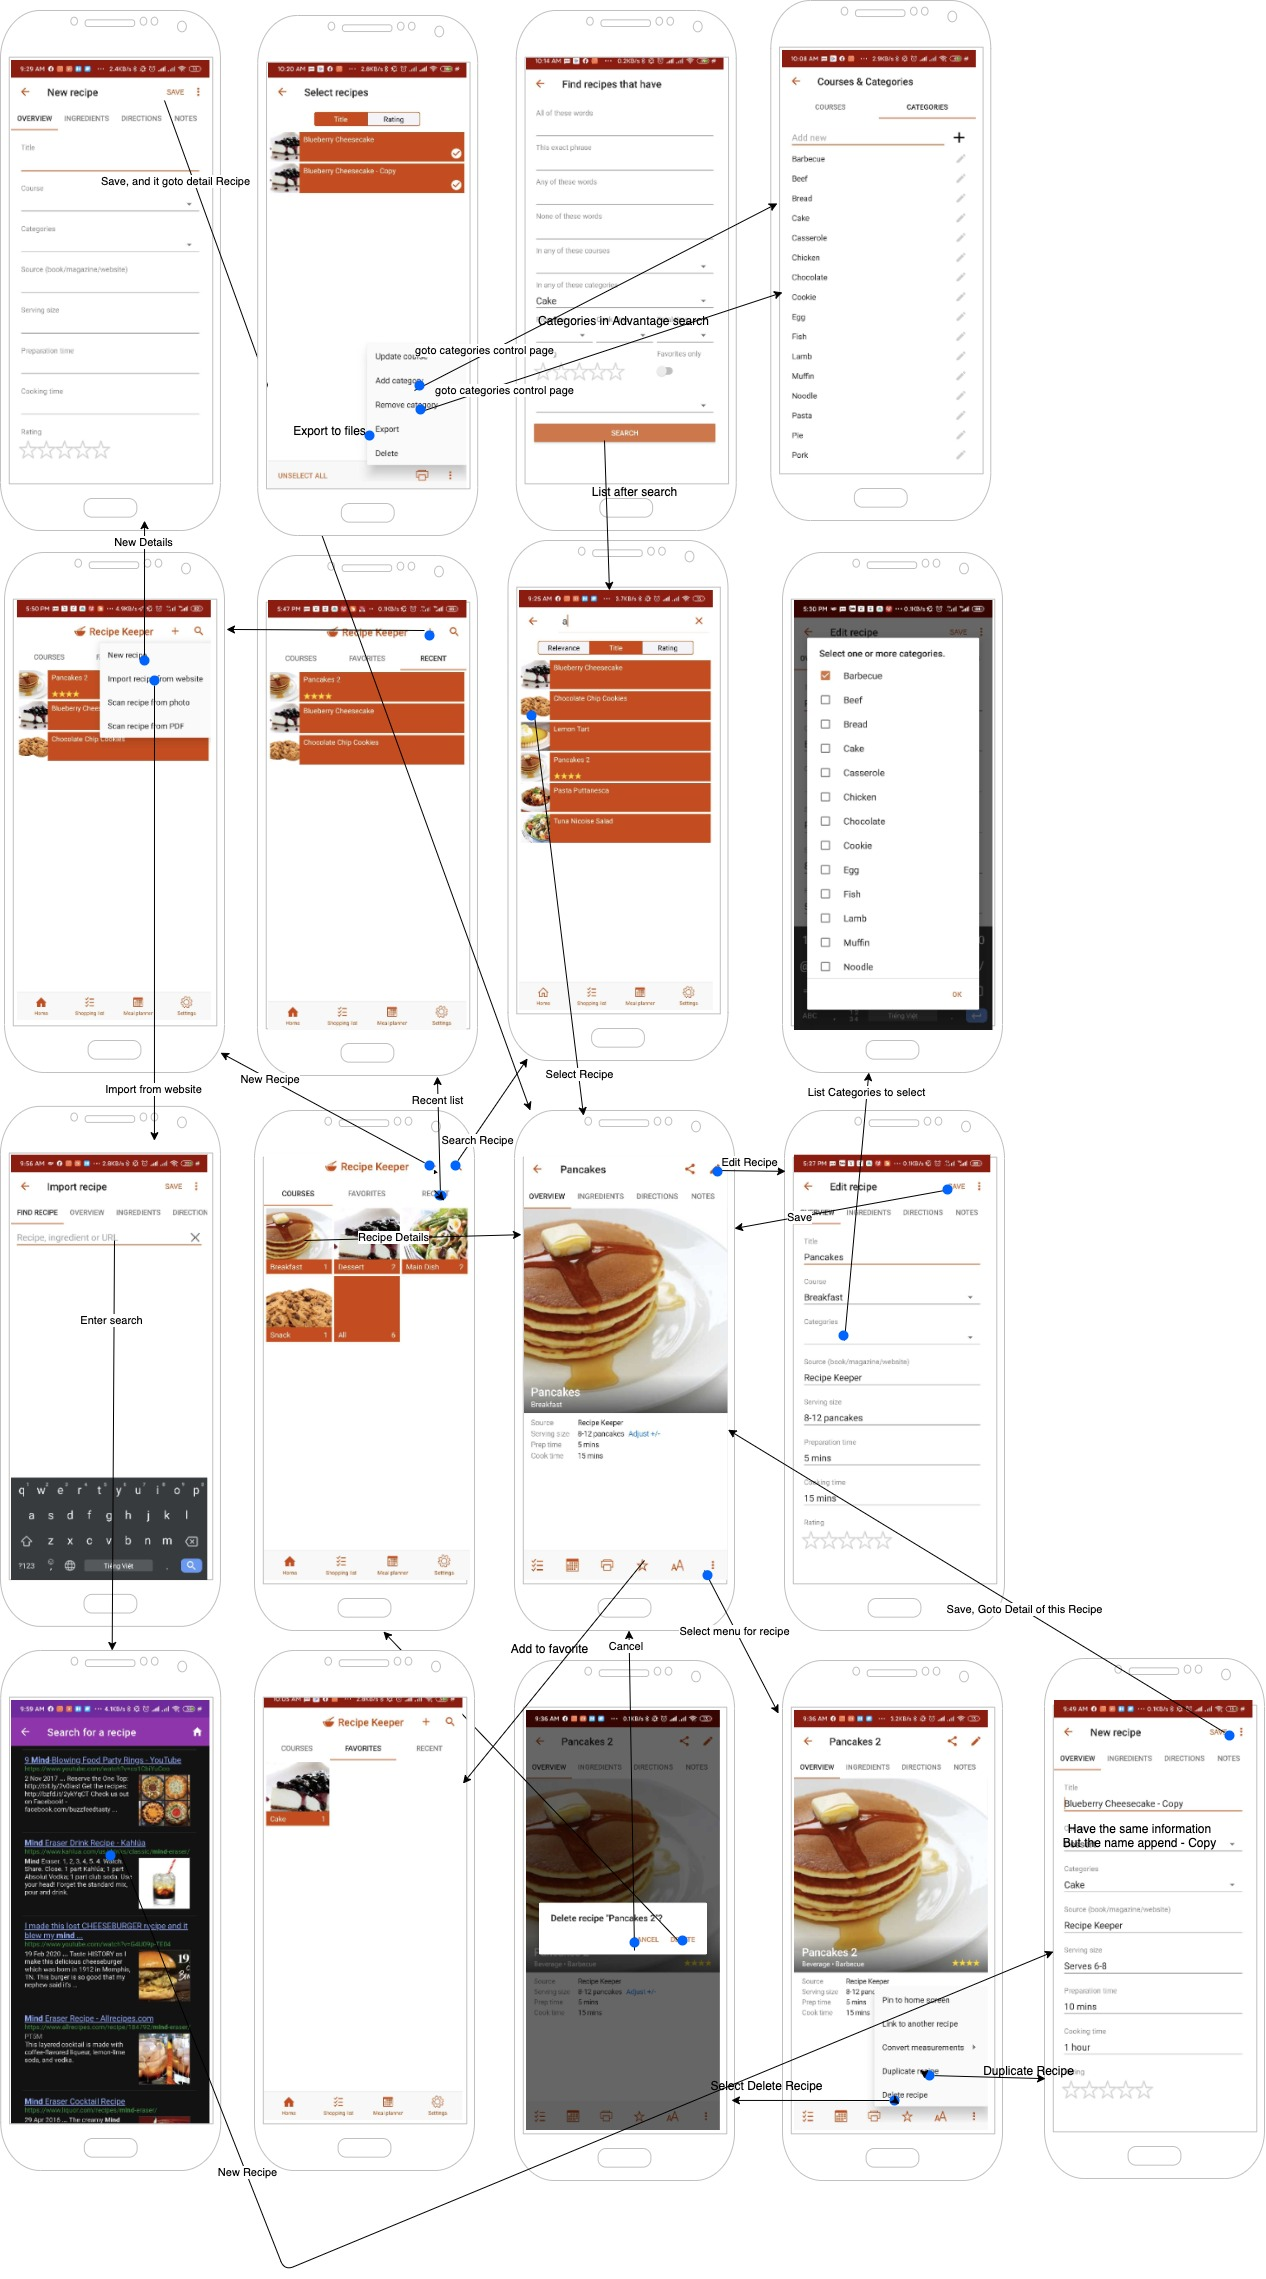
\includegraphics[scale=0.11]{Mockup.jpg}
\caption{Mockup}
\label{fig:Mockup}
\end{figure}


\subsection{ Development}

\subsection{ Rationalized development}
Rationalized development requires the use of development and analysis tools :
* Language : Flutter  
* IDE (Interface Development Environments), ex : Intellij 
* Version control software, ex: git 
* Git Repository : https://github.com/thphuc/cooking-app  
* Debuggers, ex: gdb, ddd.
* Documentation : latex.
* Tests : JUnit.

\subsection{ Test }

\subsection{ Development}

\subsection{ Development}


\subsubsection{ Solution }

\subsubsection{ IDE and tools }
\subsubsection{ Version Control }
All code and documents store with control version on GitHub, that we can manage the version of all code/documents. This is private project. \\
All member has his own branch. \\
Github url : https://github.com/thphuc/cooking-app 

\section{Conclusion }



\section{appendix }

hihi
\citep{adams1995hitchhiker}

\bibliographystyle{plain}
\bibliography{references}
\end{document}


Rationalized development requires the use of development and analysis tools :
IDE (Interface Development Environments), ex : Eclipse, Visual, NetBeans, etc.
Version control software, ex: svn, git, mercurial. Builders, ex : makefile, automake.
Debuggers, ex: gdb, ddd.
Documentation, ex : javadoc, doxygen.
Tests, ex : JUnit, CppUnit.
